\section{TVN: Electrical stimulation}
\label{sec:Stim}
\tvnnote{Torbjørn skriver dette}

\subsection{\red{TVN TO WRITE THIS}}
\begin{itemize}
\item General principle with illustration figure?
\item Only change in external potential matters, emphasizing importance of distance to electrode and electrode size.
\item Only change along neurites matter, not across membrane (electric field across membrane is already immense).
\item Activation function: Strengths and weaknesses
\item Axon terminals are main targets of action potential initiation, seen both in experiments and simulations.
\item Negative current pulses will depolarize proximal part of cell and hyperpolarize distal part of cell. Opposite for positive current.
\end{itemize}

\begin{figure}[!ht]
\begin{center}
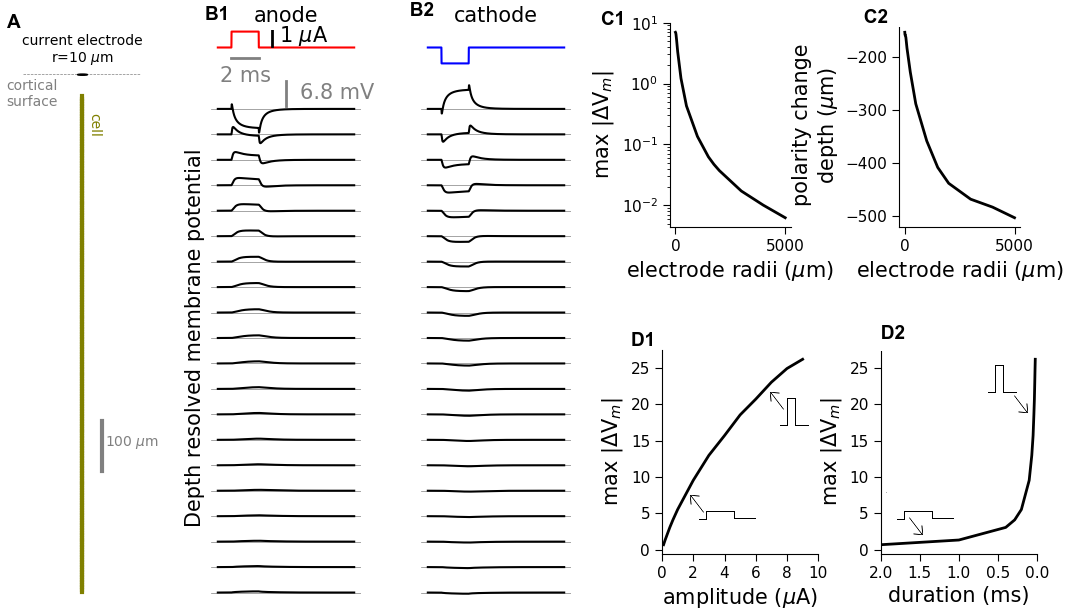
\includegraphics[width=1\textwidth]{Figures/Stim/current_stimulation_example.png}
\end{center}
\caption{\textbf{Illustration of extracellular stimulation (from cortical surface)} 
}
\label{Stim:fig:current_stimulation_example}
\end{figure}